\documentclass{article}

\usepackage{microtype}
\usepackage{graphicx}
\usepackage{subfigure}
\usepackage{booktabs}
\usepackage{hyperref}
\usepackage{multirow}

\newcommand{\theHalgorithm}{\arabic{algorithm}}

\usepackage[accepted]{icml2025}

\usepackage{amsmath}
\usepackage{amssymb}
\usepackage{mathtools}
\usepackage{amsthm}

\usepackage[capitalize,noabbrev]{cleveref}

\icmltitlerunning{HW1: Policy Gradient and Behaviour Cloning on CartPole-v1}

\begin{document}

\twocolumn[
\icmltitle{Policy Gradient Methods and Behaviour Cloning on CartPole-v1 \\
           \vspace{0.15in}
           \textnormal{\normalsize Homework 1 --- Research in LLMs, HSE x Central University}}

\begin{center}
    \textbf{Ivan A. Novosad} \\
    \texttt{inovosad@hse.ru} \\
\end{center}

\vskip 0.3in
]

% ===================================================================
\section*{About the Author}

Hi! I'm Ivan Novosad, a third-year student at HSE and a former Yandex Research 
intern (ASR team — my models are in Yandex Browser subtitles). My day job is 
efficient inference: KV cache quantization, speculative decoding, vLLM internals. 
I also have a solo paper on spatio-temporal homography alignment under review at 
IEEE Access — my first experience doing research end-to-end without co-authors.

Right now I'm working on applying GRPO to CTC-based speech recognition: generating 
hypotheses at training time the same way we do at inference, and optimizing WER 
directly through RL. That project is what brought me to this course, and why the 
RLOO $\to$ GRPO connection in Section~\ref{sec:rloo} caught my attention. This 
homework is my first hands-on RL implementation — the theory was familiar from YSDA 
courses, but debugging a policy gradient turned out to be a different experience 
entirely.

% ===================================================================
\section{Experimental Design}
\label{sec:setup}

CartPole-v1 is the assigned environment for this homework: a pole on a cart, two actions (push left/right), +1 reward per surviving timestep, up to 500 steps per episode.
The state is four-dimensional (cart position, velocity, pole angle, angular velocity), and a policy is just a binary classifier $\mathbb{R}^4 \to \{0,1\}$.
Since this is a toy task, any reasonable RL method should solve it --- which makes it useful for catching implementation bugs that harder environments would mask.

I implement six PG variants (vanilla REINFORCE, VPG + average-reward baseline, VPG + learned value baseline, RLOO, VPG + entropy regularization, VPG + value + entropy) plus behaviour cloning.
All PG methods share the same training loop; each is implemented as a separate loss callable, composable with the entropy wrapper.

The rest of this section documents the design choices I made and why.

\paragraph{Activation: tanh, not ReLU.}
I use $\tanh$ activations throughout.
ReLU dead neurons are a known issue; in PG the loss surface moves every iteration so dead neurons stay dead.
Tanh has bounded output and non-zero gradients everywhere; it is a common choice in RL.

\paragraph{Initialization: orthogonal, with small output gain.}
I use orthogonal initialization with gain $\sqrt{2}$ for hidden layers (compensating for $\tanh$'s variance contraction) and gain 0.01 for the output layer.
The small output gain produces near-zero logits and a near-uniform initial policy ($\pi \approx [0.5, 0.5]$).
This matters: if the initial policy is biased (say 90\% left), REINFORCE reinforces that bias in early episodes, and the policy can get stuck before it has explored both actions.
I found this empirically --- without the small output gain, seed~42 fails on every method.

\paragraph{Output: two logits, not one probability.}
The policy outputs two unnormalized logits passed to PyTorch's \texttt{Categorical} distribution, which handles log-probabilities, entropy, and sampling in a numerically stable way.
A single sigmoid output would require manual entropy computation and doesn't extend to $>2$ actions.

\paragraph{Separate networks and optimizers.}
Policy and value function use two independent MLPs $[4 \to 64 \to 64 \to k]$ ($k{=}2$ for policy, $k{=}1$ for value) with separate Adam optimizers ($\text{lr}_\pi = 10^{-3}$, $\text{lr}_V = 3 \times 10^{-3}$).
Shared-trunk architectures exist, but in early experiments the value loss gradients interfered with policy learning.
Separate networks avoid this, and the value function can use a higher learning rate since its regression target is more stable.

\paragraph{Greedy evaluation.}
At evaluation time I use $\arg\max$ over action probabilities.
The stochastic policy explores during training; evaluation measures what the greedy policy has learned.
Comparing with $\varepsilon$-greedy or beam-style rollouts would be interesting but is out of scope for this assignment.

\paragraph{Training details.}
I train for 1500 episodes with batches of 8 episodes per gradient update, $\gamma = 0.99$, gradient clipping at $\|\nabla\|_{\max} = 0.5$, and per-batch return normalization.
Evaluation runs every 50 episodes over 20 greedy rollouts.
``Solved'' means 5 consecutive evaluations with mean reward $\geq 475$ (i.e.\ 95\% of the maximum 500; a threshold that filters out policies that survive most but not all episodes).

Initial experiments use 5 seeds $\{42, \ldots, 46\}$.
After discovering that several claims from the 5-seed runs were not statistically supported (Section~\ref{sec:stats}), I extended all core methods plus the RLOO ablation to 15 seeds (adding seeds 47--56), and expanded the RLOO sweep from $K \in \{4, 8, 16\}$ to $K \in \{2, 3, 4, 6, 8, 12, 16, 24\}$.
BC noise robustness was tested at 5\% increments from 0\% to 100\%.

% ===================================================================
\section{A Numerical Debugging Story}
\label{sec:bug}

Before presenting results, I want to describe the most confusing part of this project.

\paragraph{Symptom.}
Every method flatlined at reward $\sim$20 (random policy level).
Gradient element variance was ${\sim}10^{-20}$.
The code ran without errors, \texttt{backward()} was called, but nothing learned.
None of the AI coding tools I tried could spot the issue either.

\paragraph{Diagnosis.}
The original implementation stored per-step log-probabilities during trajectory collection: each timestep ran a separate forward pass and saved $\log \pi_\theta(a_t | s_t)$.
These stored log-probs were later multiplied by globally-normalized returns (zero-mean by construction).

With a near-uniform initial policy (log-probs $\approx -0.693$), 500 separate forward passes accumulate independent floating-point rounding.
When multiplied by zero-mean returns and summed, the per-step contributions cancel to machine noise.

The fix: recompute all log-probabilities via a single batched \texttt{evaluate\_actions(states, actions)} call at loss time.
One GEMM produces numerically consistent log-probs.
After the fix, gradient norms went from $2.7 \times 10^{-9}$ to $2.8 \times 10^{-1}$ and VPG reached 460+ reward within 200 episodes.

The code was \emph{mathematically correct} --- REINFORCE with stored on-policy log-probs is a valid estimator.
The failure was purely numerical: catastrophic cancellation from summing many small terms with zero-mean weights.
This distinction is, in my experience, the hardest class of bugs to catch.

% ===================================================================
\section{Policy Gradient Results}
\label{sec:pg}

\subsection{What Five Seeds Showed (and What They Got Wrong)}
\label{sec:initial}

\Cref{tab:main5} summarizes the initial 5-seed comparison.
The numbers looked reasonable: VPG + Value Baseline appeared best (373.6), RLOO $K{=}8$ was competitive (350.4), entropy seemed to help reliability (4/5 $\to$ 5/5 solve rate for entropy ablations in \Cref{tab:entropy}), and the value baseline appeared to reduce gradient variance by 18\%.

\begin{table}[h]
\caption{Initial 5-seed comparison. These rankings do not survive 15-seed testing (see~\Cref{tab:paired}).}
\label{tab:main5}
\centering
\small
\begin{tabular}{lccc}
\toprule
\textbf{Method} & \textbf{Reward} & \textbf{Std} & \textbf{Solved} \\
\midrule
VPG                   & 351.1 & 122.0 & 4/5 \\
VPG + Avg Baseline    & 320.4 & 103.7 & 4/5 \\
VPG + Value Baseline  & 373.6 & 112.2 & 4/5 \\
RLOO $K{=}8$          & 350.4 & 115.9 & 4/5 \\
VPG + Entropy         & 327.4 & 105.2 & 4/5 \\
VPG + Value + Entropy & 336.5 & 115.2 & 4/5 \\
\bottomrule
\end{tabular}
\end{table}

\begin{figure}[h]
\centering
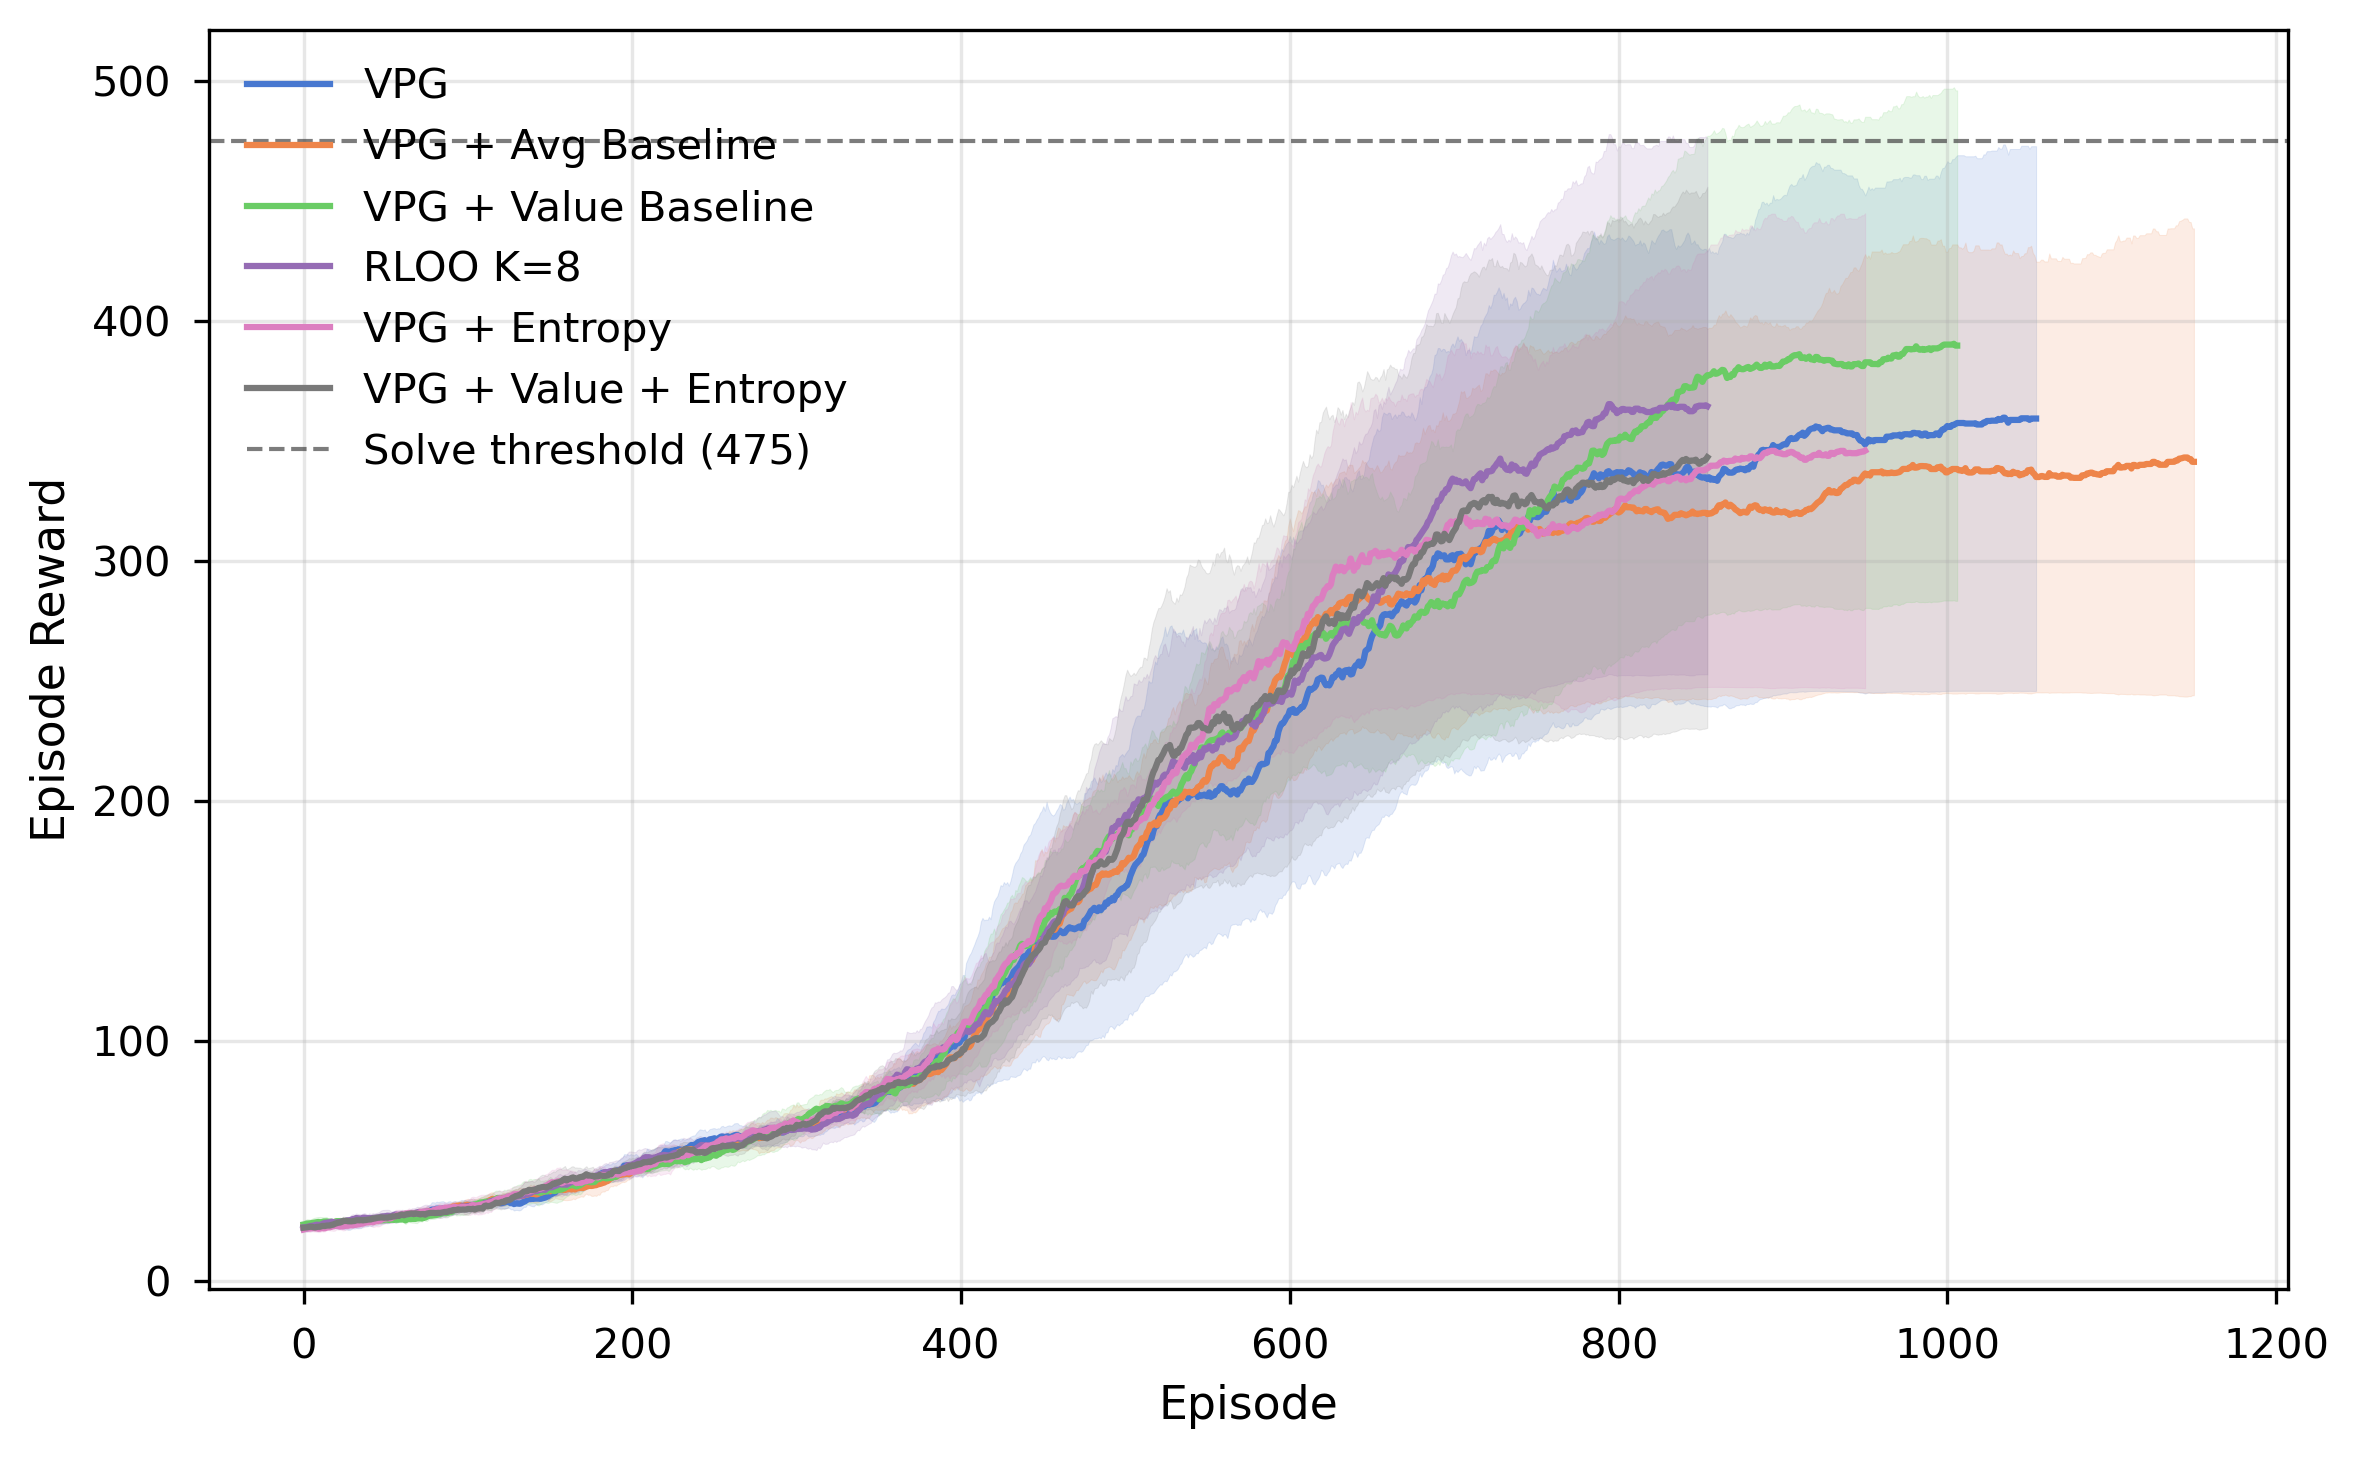
\includegraphics[width=\columnwidth]{figures/fig1_learning_curves.png}
\caption{Training curves for 6 PG variants, 5 seeds, 50-episode rolling average with $\pm 1$ std shading.
All methods are indistinguishable before episode 400.}
\label{fig:learning}
\end{figure}

Looking at the learning curves (\Cref{fig:learning}), all six methods are indistinguishable before episode 400 and diverge only in late training, with high cross-seed variance.
This immediately raised a question: are these differences real, or just noise from 5 seeds?
One pattern stands out: \textbf{seed~42 fails for every single method}.
The divergence between methods in late training is initialization-dependent, not method-dependent.
This was the first sign that 5 seeds might not be enough to claim anything.

\subsection{Statistical Reality Check}
\label{sec:stats}

I ran 10 additional seeds (47--56) for all core methods and RLOO $K$ configurations, giving 15 seeds per method.
\Cref{tab:paired} reports seed-matched paired $t$-tests.

\begin{table}[h]
\caption{Paired comparisons (15 seeds). Only RLOO and entropy+value reach significance.}
\label{tab:paired}
\centering
\small
\begin{tabular}{lcccl}
\toprule
\textbf{Comparison} & $\Delta$ & $p$ & $d$ & \textbf{Verdict} \\
\midrule
Value vs VPG        & $-1.1$  & 0.91  & $-0.01$ & null \\
Avg vs VPG          & $-13.6$ & 0.42  & $-0.16$ & null \\
V+Ent vs Value      & $-40.3$ & \textbf{0.010} & $-0.54$ & hurts \\
RLOO $K{=}4$ vs VPG & $+51.7$ & \textbf{0.010} & $+0.82$ & helps \\
\bottomrule
\end{tabular}
\end{table}

The short answer: baselines don't help on CartPole.

The value baseline shows zero effect (\Cref{tab:paired}: $p = 0.91$, CI includes zero in both directions).
The average-reward baseline is similarly null ($p = 0.42$).
The ``18\% gradient variance reduction'' from the value baseline also disappears with 15 seeds; the confidence intervals overlap completely (Section~\ref{sec:gradvar}).

Two effects are real.
RLOO $K{=}4$ outperforms VPG ($p = 0.010$, $d = 0.82$, CI entirely above zero).
And adding entropy to VPG + Value \emph{hurts} ($p = 0.010$, $d = -0.54$).
I see two possible explanations. First, the entropy bonus adds an opposing term to the policy gradient, which simply slows convergence; with a fixed 1500-episode budget, slower convergence means lower final reward. Second, the entropy pressure may destabilize the value function: $V(s)$ tries to track $\mathbb{E}[G_t | s]$ while the policy keeps shifting toward uniform, making advantage estimates noisy. I cannot distinguish these from the current data.

I also tested whether entropy improves solve reliability.
With 5 seeds, entropy methods solved 5/5 versus 4/5 for non-entropy.
With 15 seeds: entropy solves 28/30, non-entropy solves 42/45 (Fisher exact $p = 1.0$).
Not significant.
The initial observation was driven entirely by seed~42.

\paragraph{Why baselines don't help here.}
CartPole has a bimodal reward distribution: episodes either fail quickly ($\sim$20 reward) or succeed ($\sim$500).
The raw return $G_t$ already carries strong signal (``this trajectory succeeded'' or ``this trajectory failed''), and subtracting a baseline from that doesn't reduce variance much.
This makes sense — baselines help when per-state value estimates carry information. Here the return is basically binary.
CartPole is below that complexity threshold.

This is an honest null result, not a failure.
I can implement baselines correctly (the code works, the math is right), but the environment is too simple for them to matter.

\subsection{RLOO: Update Frequency Dominates}
\label{sec:rloo}

I swept $K \in \{2, 3, 4, 6, 8, 12, 16, 24\}$ with 15 seeds each (\Cref{tab:rloo}, \Cref{fig:rloo}).

\begin{figure}[h]
\centering
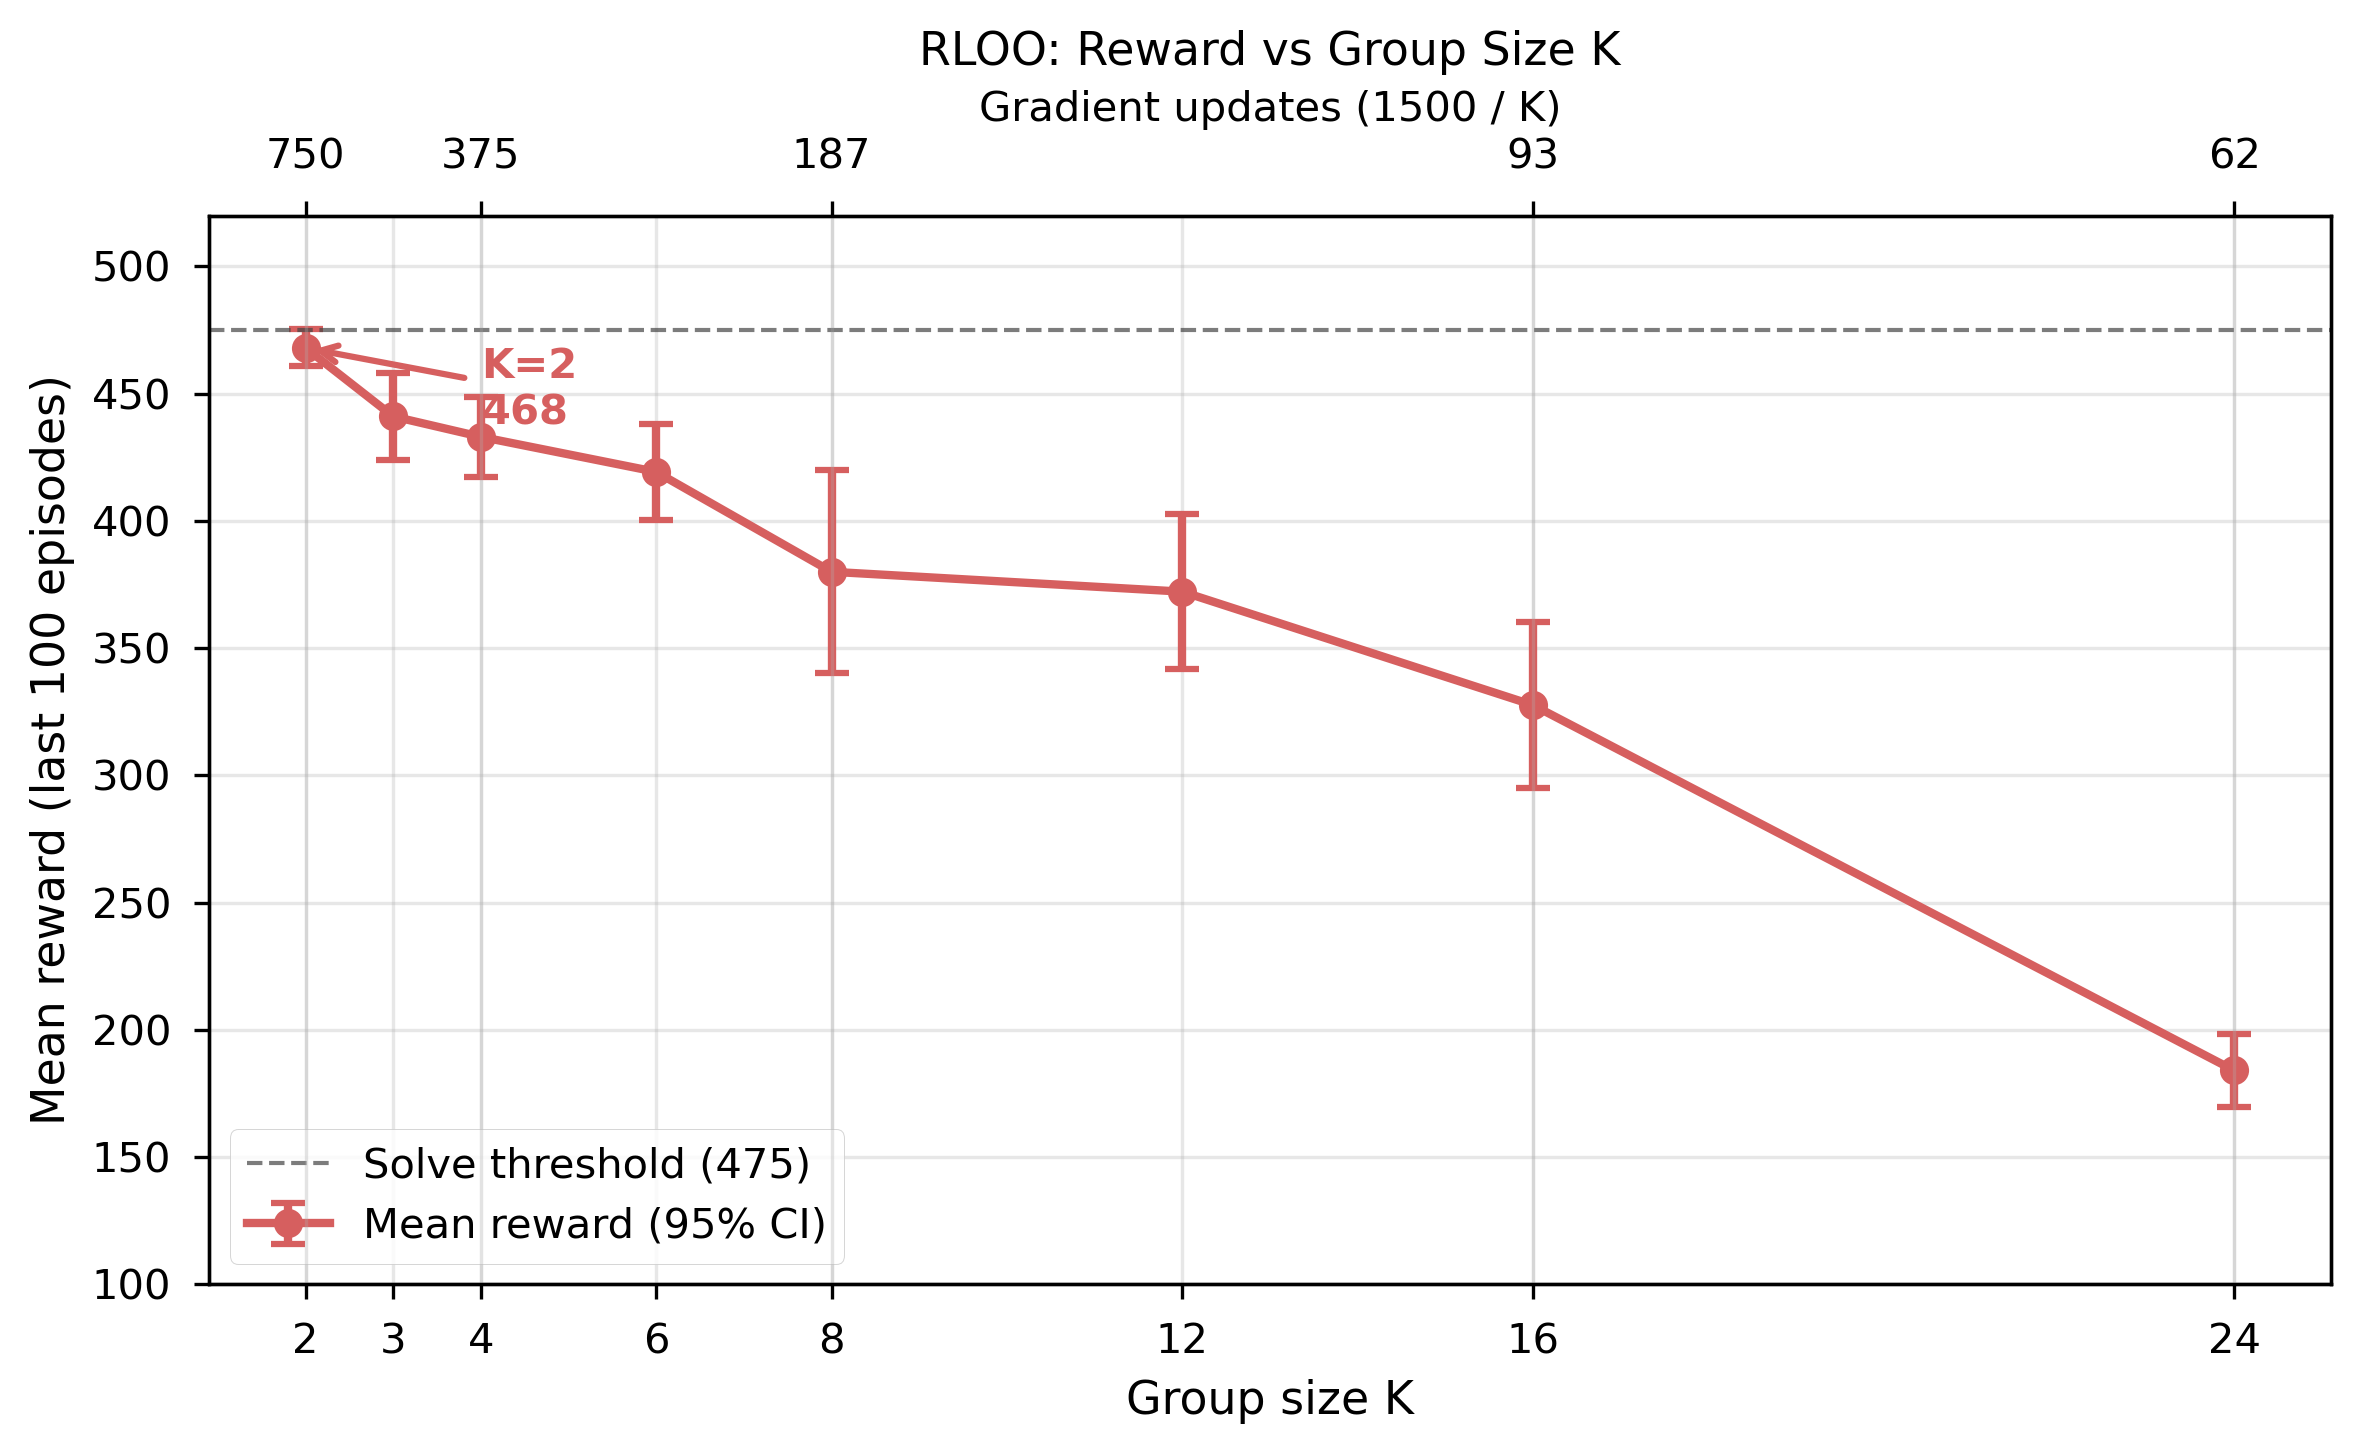
\includegraphics[width=\columnwidth]{figures/fig9_rloo_curve.png}
\caption{RLOO reward vs group size $K$ (15 seeds per point, 95\% CIs).
Top axis: gradient update count ($1500/K$).
Reward decreases monotonically with $K$.}
\label{fig:rloo}
\end{figure}

\begin{table}[h]
\caption{RLOO $K$ ablation (15 seeds). CIs: mean $\pm$ 1.96 $\cdot$ std$/\sqrt{15}$.}
\label{tab:rloo}
\centering
\small
\begin{tabular}{rrrrcr}
\toprule
$K$ & Updates & Reward & 95\% CI & Std & Solved \\
\midrule
2  & 750 & \textbf{468.0} & $[460.7, 475.3]$ & \textbf{14.3} & 15/15 \\
3  & 500 & 441.1 & $[423.9, 458.3]$ & 34.1 & 15/15 \\
4  & 375 & 433.1 & $[417.3, 448.9]$ & 31.1 & 15/15 \\
6  & 250 & 419.3 & $[400.4, 438.2]$ & 37.4 & 15/15 \\
8  & 188 & 380.0 & $[340.1, 419.9]$ & 78.8 & 14/15 \\
12 & 125 & 372.2 & $[341.8, 402.6]$ & 60.0 & 15/15 \\
16 & 94  & 327.7 & $[295.2, 360.2]$ & 64.3 & 15/15 \\
24 & 63  & 184.1 & $[169.6, 198.6]$ & 28.6 & 2/15 \\
\bottomrule
\end{tabular}
\end{table}

Reward decreases monotonically with $K$ (Spearman $\rho = -0.80$, $p < 10^{-27}$).
The winner is $K{=}2$ --- the noisiest possible LOO baseline, computed from a single other trajectory --- at 468.0, the highest reward of any configuration I tested.

I think this is because of update frequency: under a fixed 1500-episode budget, $K{=}2$ gets 750 gradient updates versus 63 for $K{=}24$.
For CartPole, where the reward signal is essentially binary (fail or succeed), even a one-trajectory baseline is informative.
Update frequency dominates baseline quality completely.

$K{=}24$ is catastrophic: 184.1 mean reward, only 2/15 solved.
63 gradient updates is simply not enough to train a policy.
$K{=}8$ shows anomalously high variance (std = 78.8) and the only sub-100\% solve rate among $K \leq 16$, suggesting a fragile regime where neither the baseline quality nor the update count is sufficient.

\paragraph{A note on GRPO.}
I mention this because I am currently working on GRPO for ASR at Yandex Research, and the parallel is hard to ignore.
GRPO samples $G$ completions per prompt and computes advantages relative to the group, which is essentially RLOO for LLM training.
The \texttt{num\_generations} parameter plays the same role as $K$ here.
If update frequency dominates even with a maximally noisy baseline, smaller group sizes deserve consideration when the reward signal is clean.

\paragraph{Wall-clock cost.}
RLOO $K{=}2$ is also the \emph{fastest} configuration at 14.9s per run, 
compared to 15.8s for $K{=}4$ and 20.9s for vanilla VPG. Fewer, larger 
batches amortize Python-level overhead and GPU kernel launch costs. The 
method that learns best also trains fastest.

\subsection{Entropy Regularization}
\label{sec:entropy}

The entropy ablation (\Cref{tab:entropy}) sweeps $\beta \in \{0.001, 0.01, 0.05, 0.1\}$ with linear schedule, and three schedules at $\beta{=}0.01$.
These are 5-seed results; I did not extend them to 15 seeds because the cross-method entropy comparison (Section~\ref{sec:stats}) already showed that entropy's aggregate benefit is not significant.

\begin{table}[h]
\caption{Entropy ablation (5 seeds).}
\label{tab:entropy}
\centering
\small
\begin{tabular}{rllcc}
\toprule
$\beta$ & Schedule & Reward & Entropy & Solved \\
\midrule
0.001 & linear   & 378.4 & 0.528 & 5/5 \\
0.01  & linear   & 375.9 & 0.536 & 5/5 \\
0.05  & linear   & 317.5 & 0.549 & 5/5 \\
0.1   & linear   & 360.2 & 0.556 & 5/5 \\
\midrule
0.01  & constant & 350.8 & 0.539 & 5/5 \\
0.01  & linear   & \textbf{398.2}$^\dagger$ & 0.528 & 5/5 \\
0.01  & cosine   & 391.1 & 0.533 & 5/5 \\
\bottomrule
\end{tabular}
\end{table}

\begin{figure}[h]
\centering
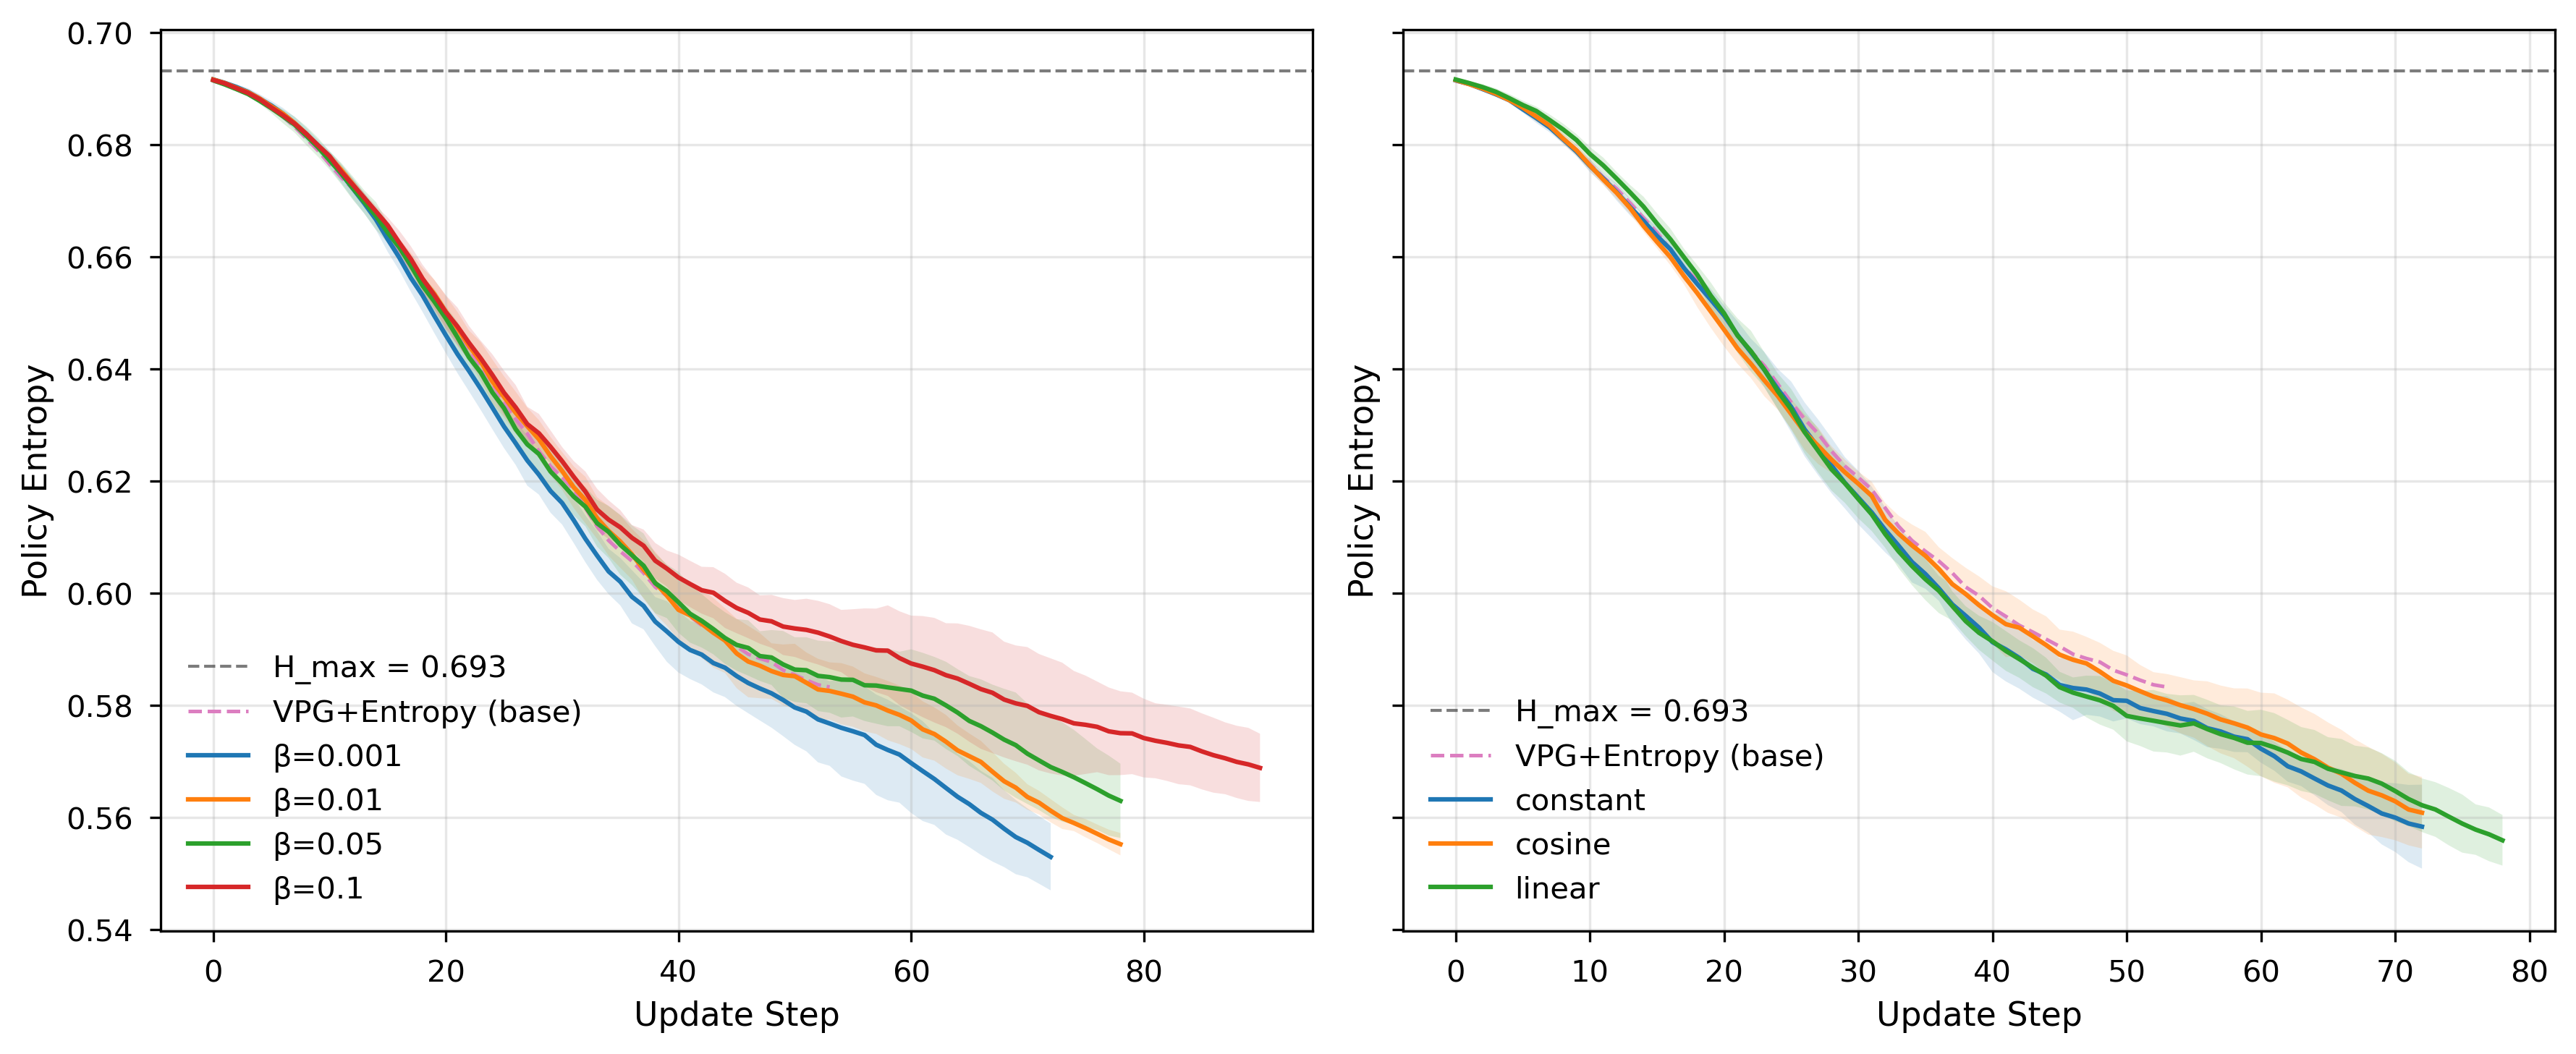
\includegraphics[width=\columnwidth]{figures/fig3_entropy.png}
\caption{Policy entropy over training. Left: $\beta$ sweep. Right: schedule comparison. $^\dagger$Same hyperparameters as row 2 of the $\beta$ sweep (375.9); the 22-point gap is cross-run seed variance, illustrating why 5-seed comparisons are unreliable.}
\label{fig:entropy}
\end{figure}

Within entropy configurations, the linear schedule ($\beta{=}0.01$) achieves the best result at 398.2 $\pm$ 32.2, beating constant by 47 points.
The linear schedule provides high exploration pressure early and decays to near-zero, allowing full exploitation in late training.
Constant schedule maintains unnecessary entropy pressure throughout.

The $\beta$ relationship is non-monotonic: $\beta{=}0.05$ performs worst (317.5), sitting in a dead zone where entropy pressure is strong enough to slow convergence but too weak to fundamentally change exploration.

\subsection{Gradient Variance: A Null Result}
\label{sec:gradvar}

\begin{figure}[h]
\centering
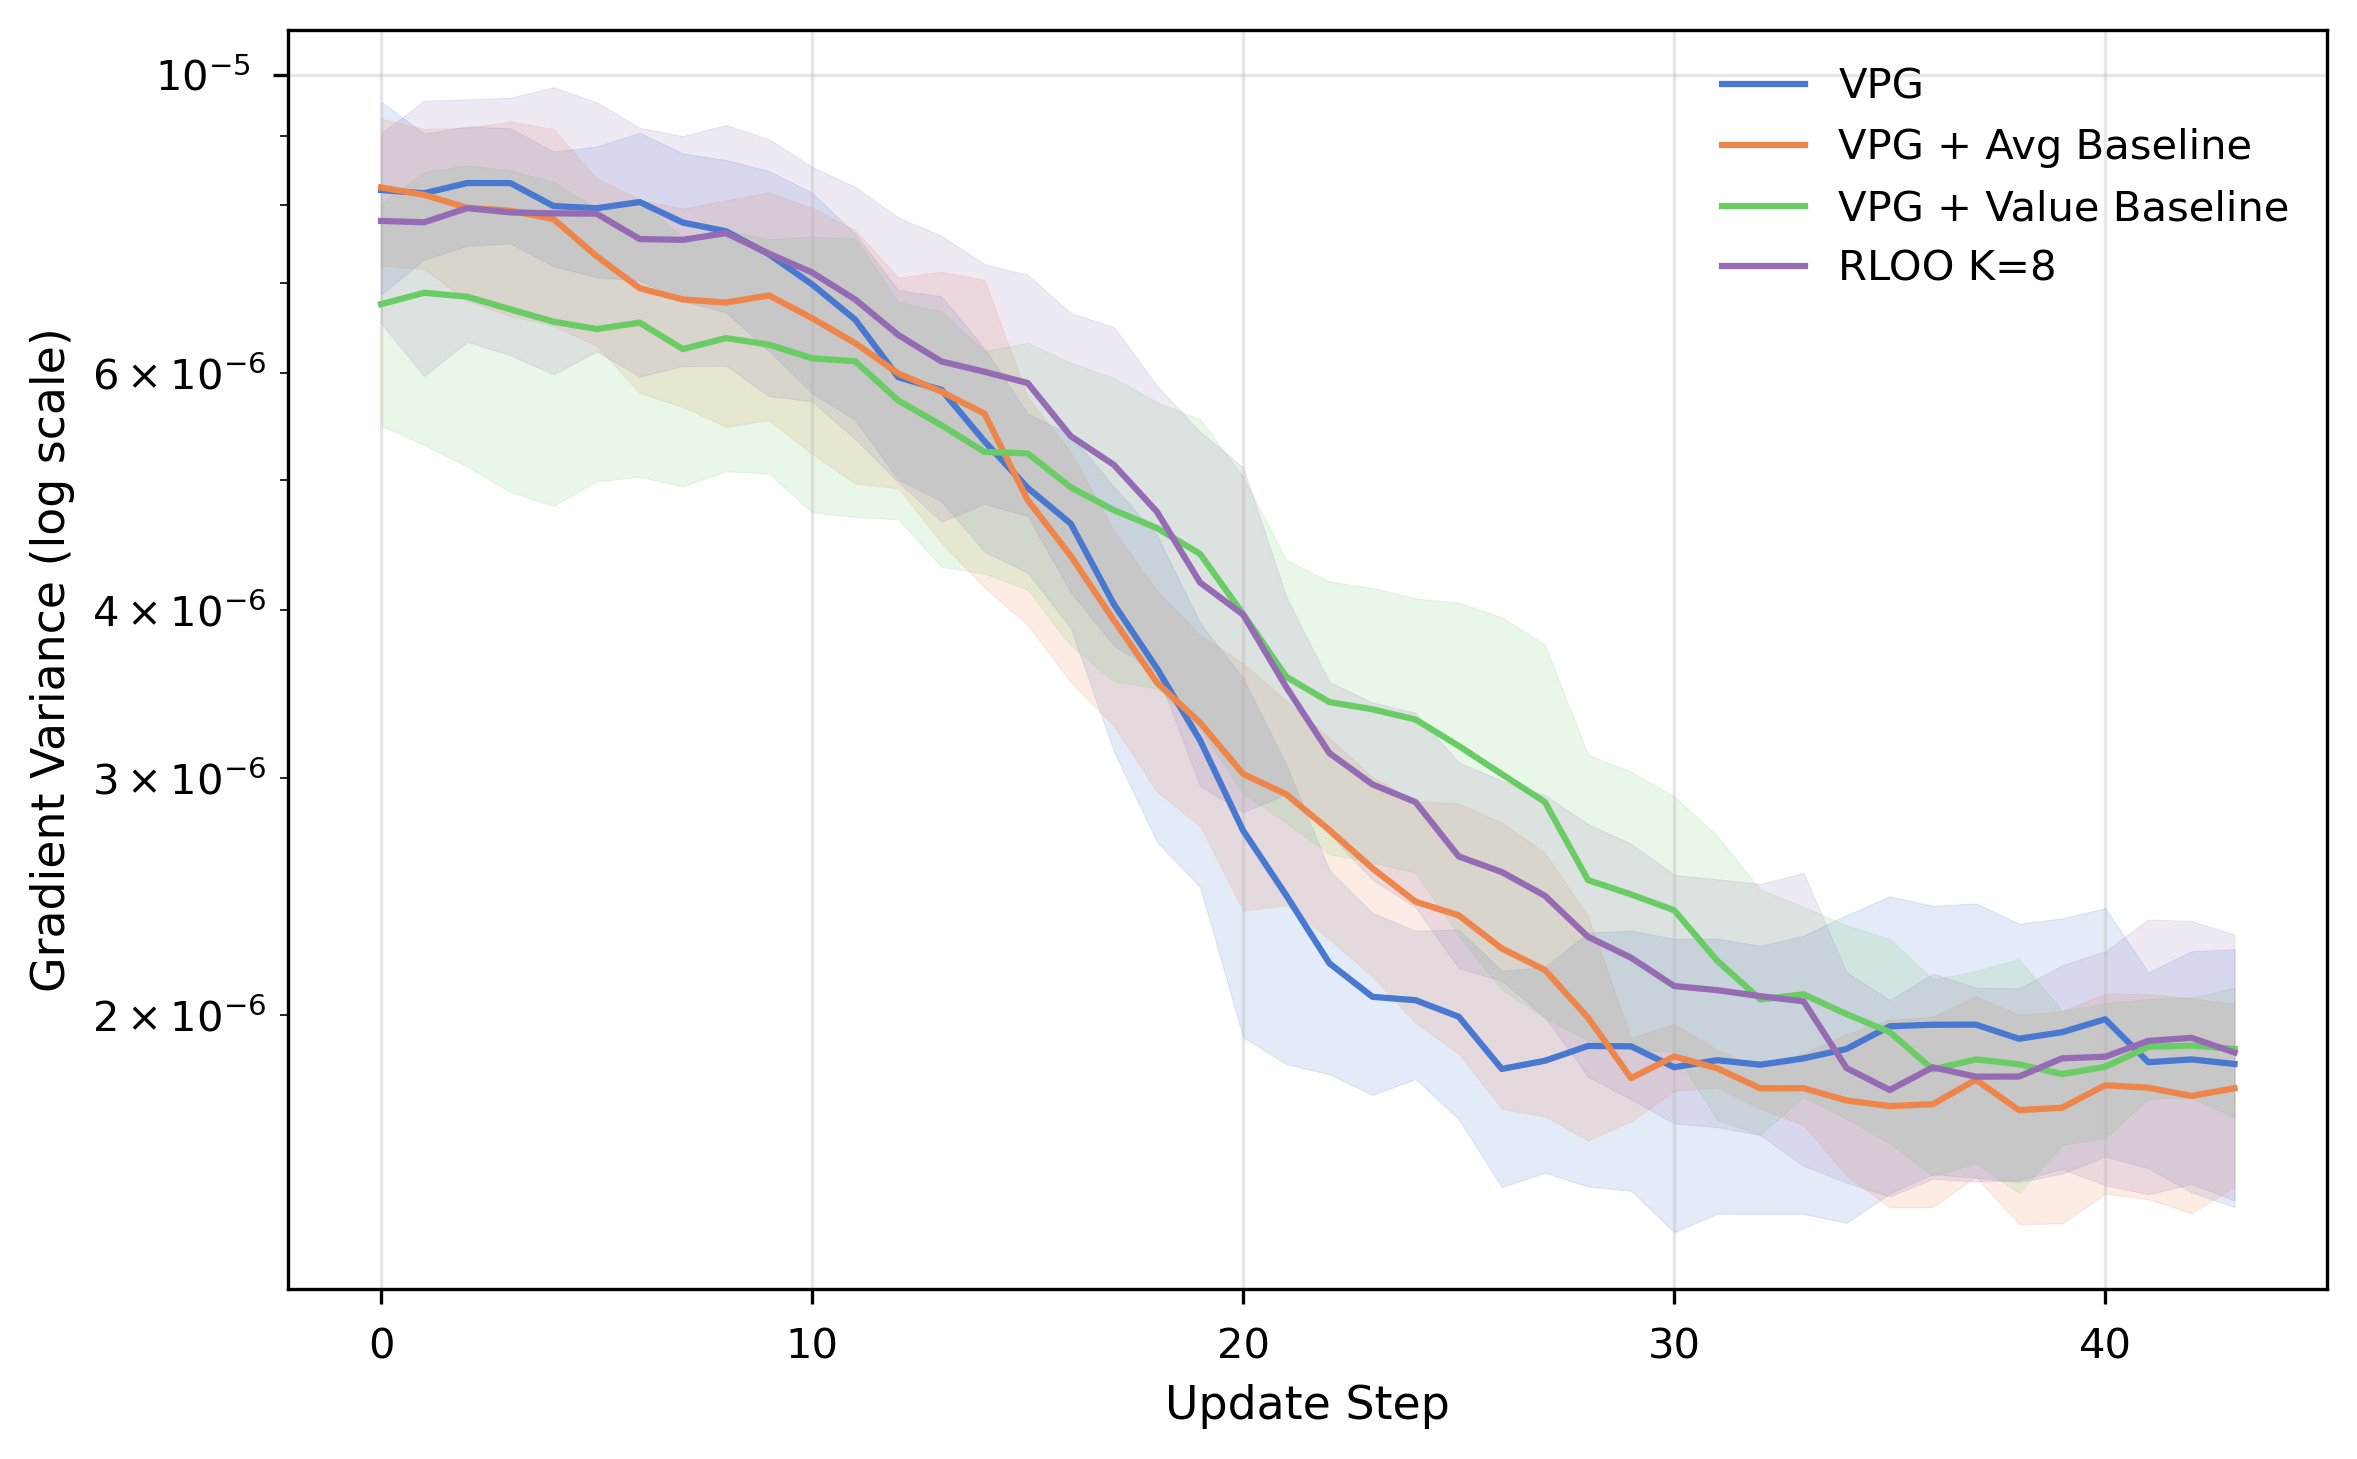
\includegraphics[width=\columnwidth]{figures/fig2_grad_variance.png}
\caption{Per-update gradient element variance (log scale), 5 seeds.}
\label{fig:gradvar}
\end{figure}

I had a research idea: baselines are supposed to reduce the variance of the policy gradient estimator, but do they also stabilize the gradient flow in a more general sense, lowering the variance of gradient \emph{elements} across parameters?
If so, that would be a non-trivial insight about optimization dynamics beyond the standard variance-reduction argument.

I tracked per-update gradient element variance (\Cref{fig:gradvar}).
To be clear: this is not the REINFORCE estimator variance (across trajectory samples), but the variance of elements within a single gradient vector, i.e.\ how uniformly the gradient is distributed across parameters.

The answer: no.
With 15 seeds, the four baseline methods (VPG, Avg, Value, Value+Entropy) show no significant differences in early-training variance (all CIs overlap). RLOO $K{=}4$ is the exception: its early variance is ${\sim}1.5\times$ higher ($1.02 \times 10^{-5}$, CI $[8.98, 11.48] \times 10^{-6}$) than the others, likely because the LOO estimator on small groups produces noisier per-update gradients.

All methods show a universal 5--8$\times$ reduction from early to late training as the policy converges.
This is about policy convergence, not method differences.

% ===================================================================
\section{Behaviour Cloning}
\label{sec:bc}

The expert policy (VPG + Value + Entropy, trained to convergence) achieves $500.0 \pm 0.0$ over 100 evaluation episodes.

\subsection{Dataset Size: A Phase Transition}
\label{sec:bc_size}

\begin{figure}[h]
\centering
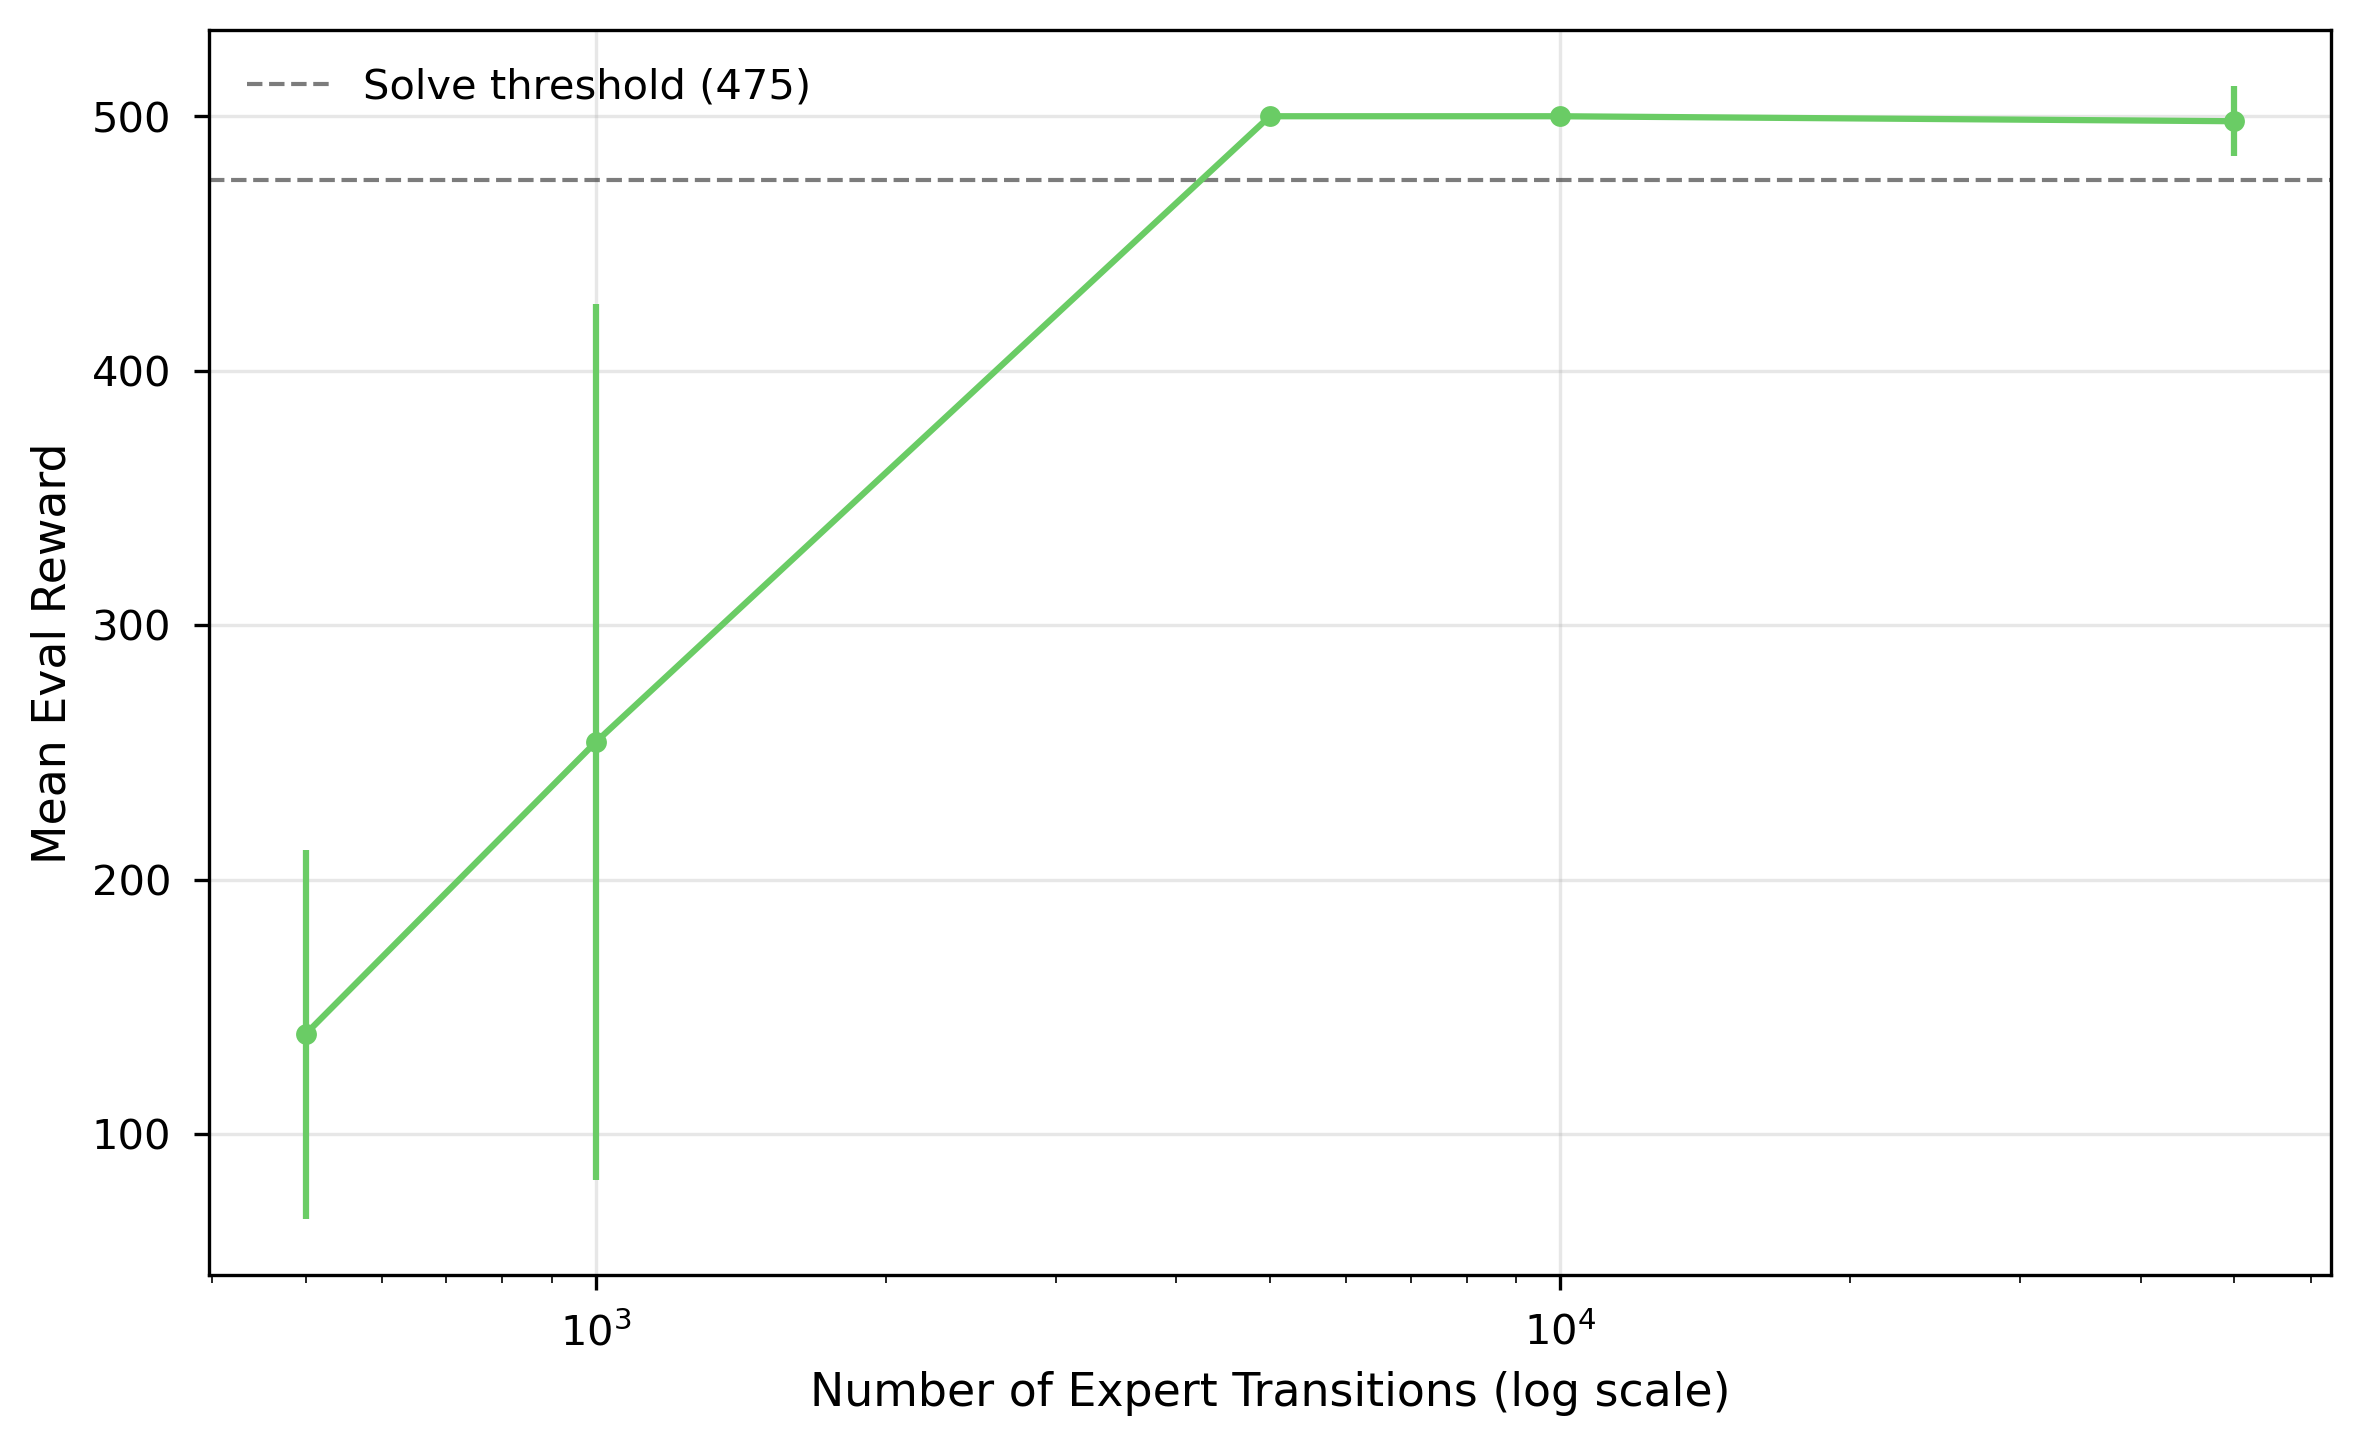
\includegraphics[width=\columnwidth]{figures/fig5_bc_dataset_size.png}
\caption{BC reward vs number of expert transitions (log scale).}
\label{fig:bc_size}
\end{figure}

BC performance has a sharp phase transition between 1,000 and 5,000 transitions (\Cref{tab:bc_size}, \Cref{fig:bc_size}).
At 500 transitions: 139.2.
At 5,000: 500.0 (perfect).
I should note that the grid (500, 1k, 5k, 10k) is sparse in the transition zone, so I cannot pinpoint the exact threshold; it is somewhere between 1k and 5k.
A denser sweep (e.g.\ 2k, 3k, 4k) would narrow this down.

\begin{table}[h]
\caption{BC vs dataset size. Expert achieves 500.0.}
\label{tab:bc_size}
\centering
\small
\begin{tabular}{rccc}
\toprule
\textbf{Transitions} & \textbf{Reward} & \textbf{Std} & \textbf{Gap} \\
\midrule
500    & 139.2 & 72.5  & 360.8 \\
1,000  & 254.0 & 172.1 & 246.0 \\
5,000  & \textbf{500.0} & \textbf{0.0} & 0.0 \\
10,000 & 500.0 & 0.0   & 0.0 \\
\bottomrule
\end{tabular}
\end{table}

CartPole's policy is a simple function ($\mathbb{R}^4 \to \{0,1\}$), so the relevant decision boundary in 4D state space can be fully covered by $\sim$5,000 diverse transitions.
Below this threshold, there are regions where the classifier has no training signal and makes random predictions.

\subsection{Distribution Shift: Compounding Errors in Action}
\label{sec:bc_shift}

\begin{figure}[h]
\centering
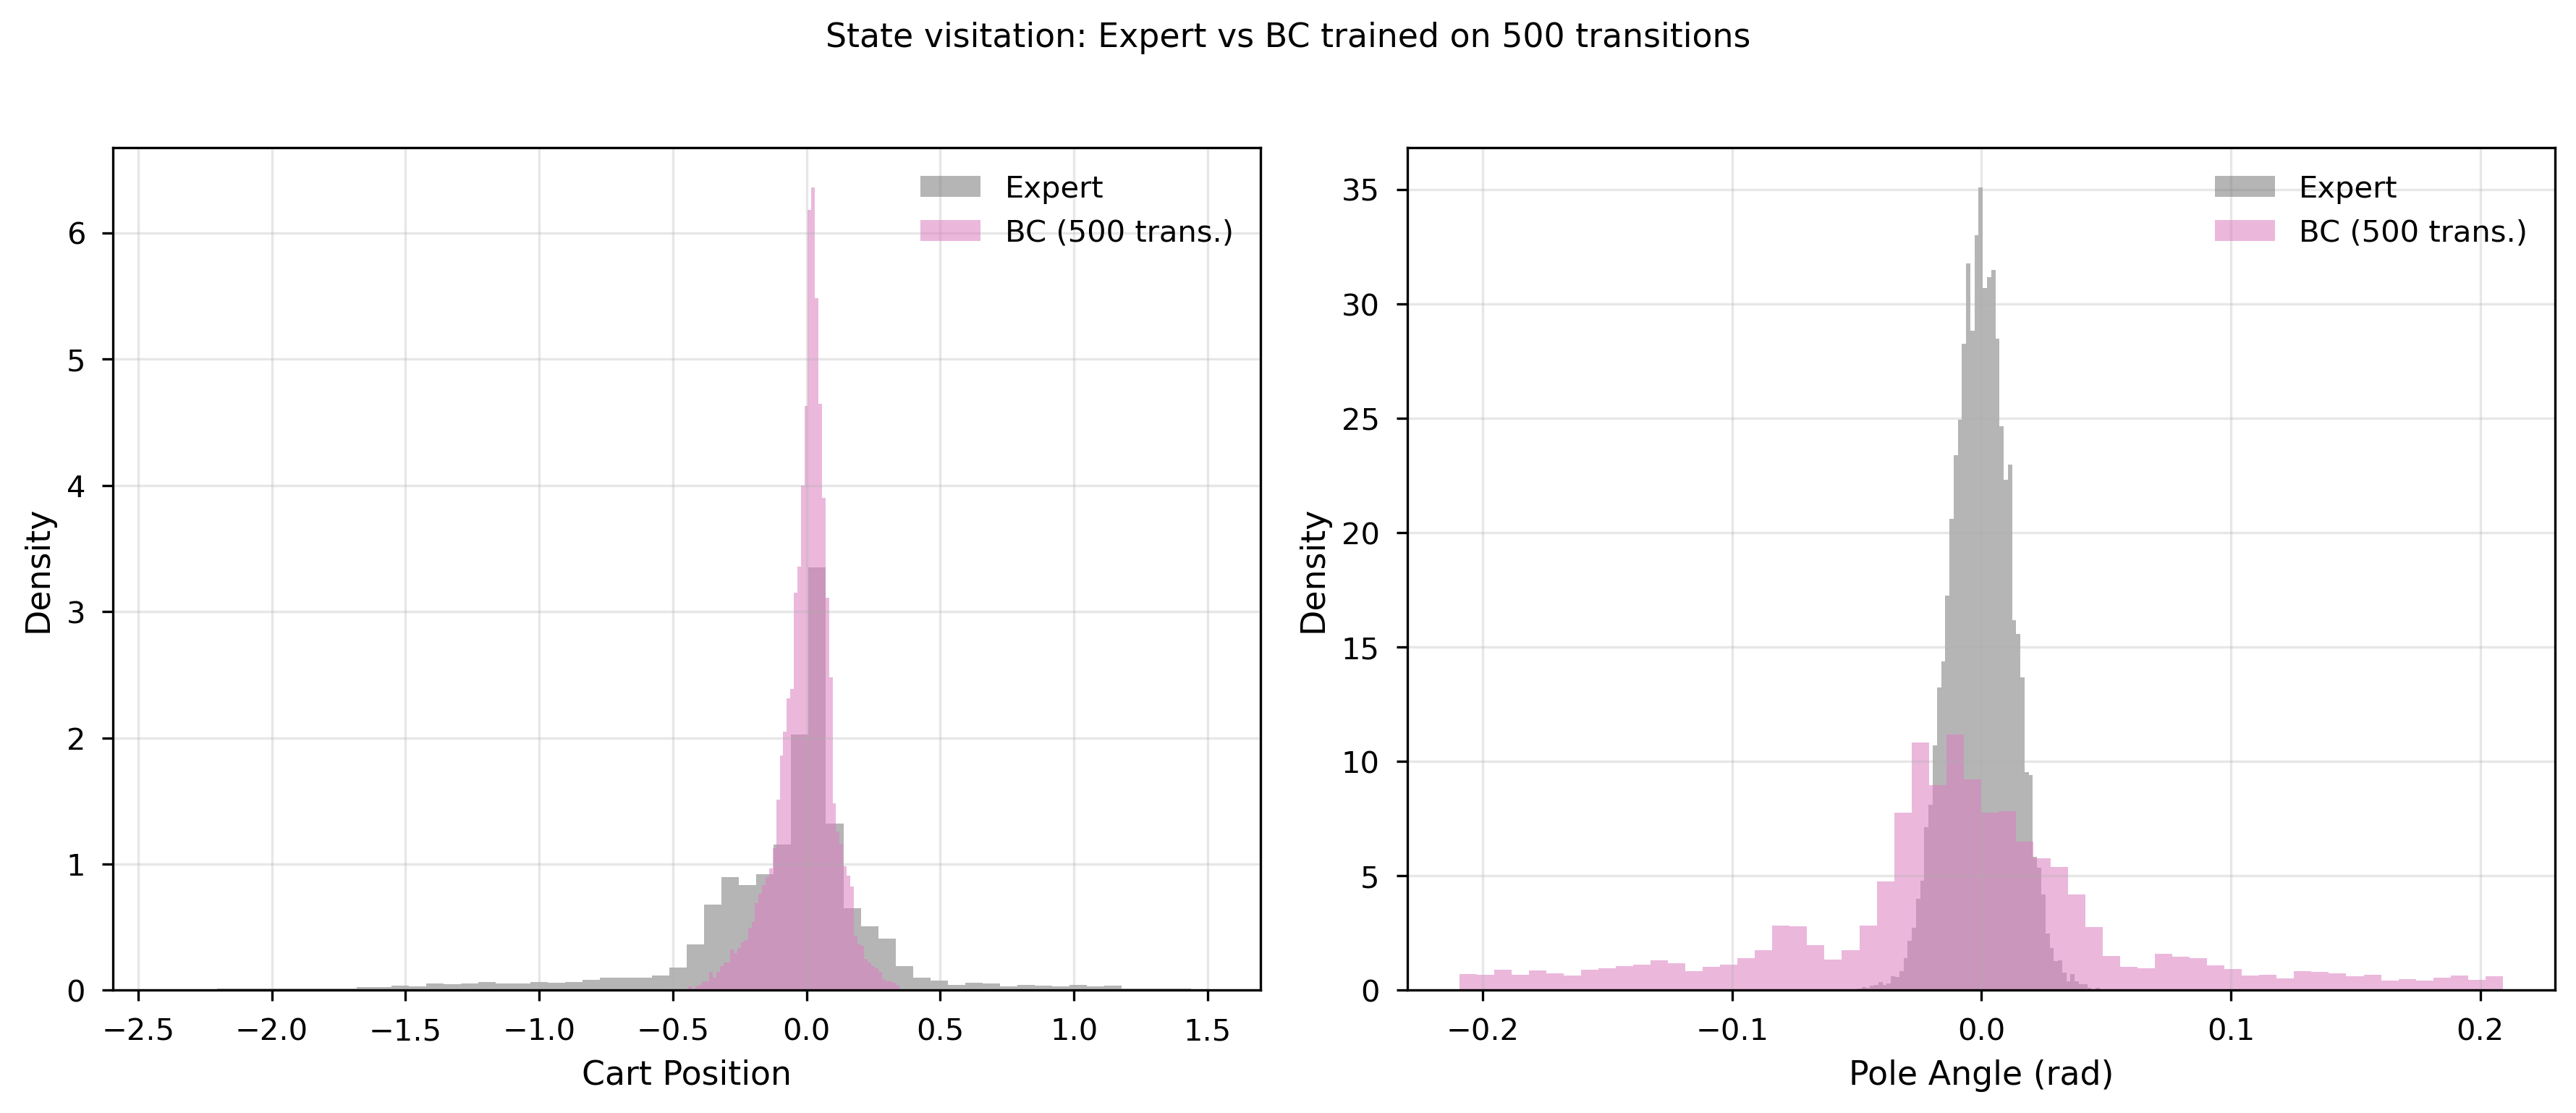
\includegraphics[width=\columnwidth]{figures/fig6_bc_state_dist.png}
\caption{State visitation: expert vs BC (500 transitions). The clone visits pole angles up to $\pm 0.2$~rad, far outside the expert's tight distribution.}
\label{fig:bc_dist}
\end{figure}

\begin{figure}[h]
\centering
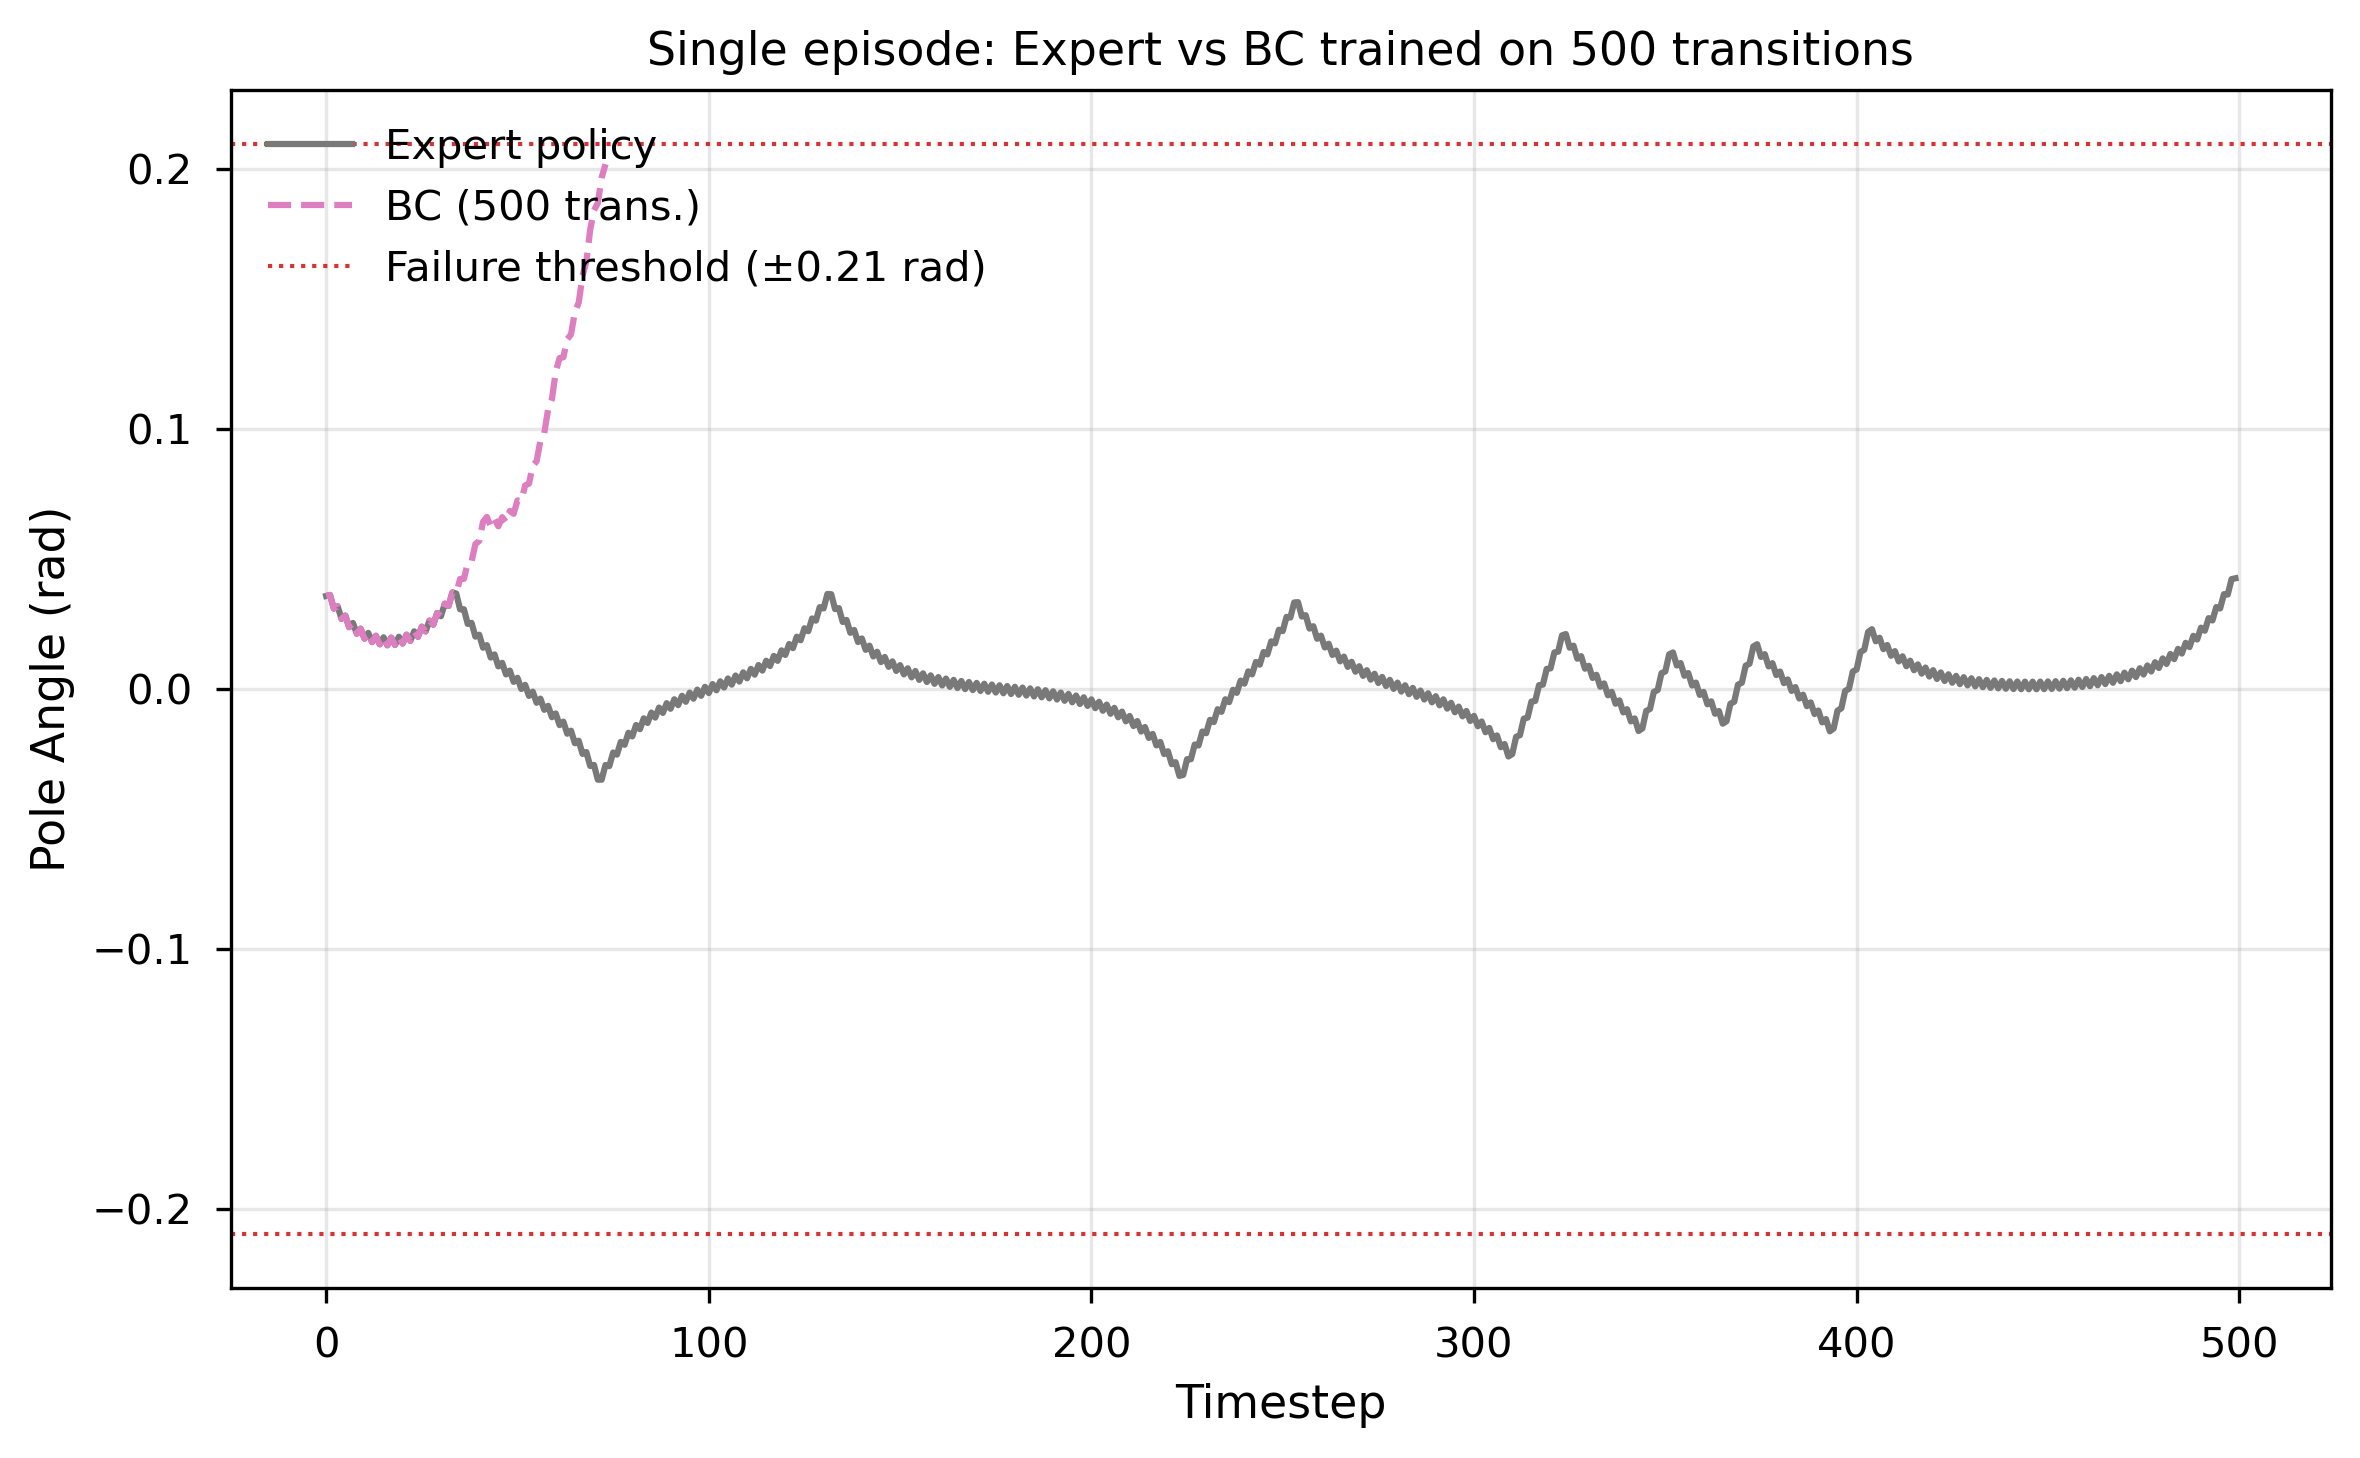
\includegraphics[width=\columnwidth]{figures/fig7_bc_failure_episode.png}
\caption{Single episode: BC (500 transitions) tracks the expert for $\sim$30 steps, then diverges and fails.}
\label{fig:bc_fail}
\end{figure}

Figures~\ref{fig:bc_dist} and~\ref{fig:bc_fail} show the compounding error mechanism.
The histogram (\Cref{fig:bc_dist}) is telling: the 500-transition clone develops heavy tails in pole angle, visiting $\pm 0.2$~rad states that never appear in the expert's distribution.
In a single episode, the clone tracks the expert for about 30 steps, then a small error cascades: it enters OOD (out-of-distribution) states, picks wrong actions, and spirals.
This matches the theoretical $O(\varepsilon T^2)$ compounding bound, where per-step imitation error $\varepsilon$ grows quadratically over horizon $T$.

On-policy RL avoids this by construction: the policy always trains on states it actually visits.

\subsection{Noise Robustness: A Sigmoid and a Surprise}
\label{sec:bc_noise}

I tested BC across 21 noise levels from 0\% to 100\% in 5\% increments, with 5 seeds for the transition zone (20--50\%).
The result (\Cref{fig:bc_noise}) is cleaner than I expected.

\begin{figure}[h]
\centering
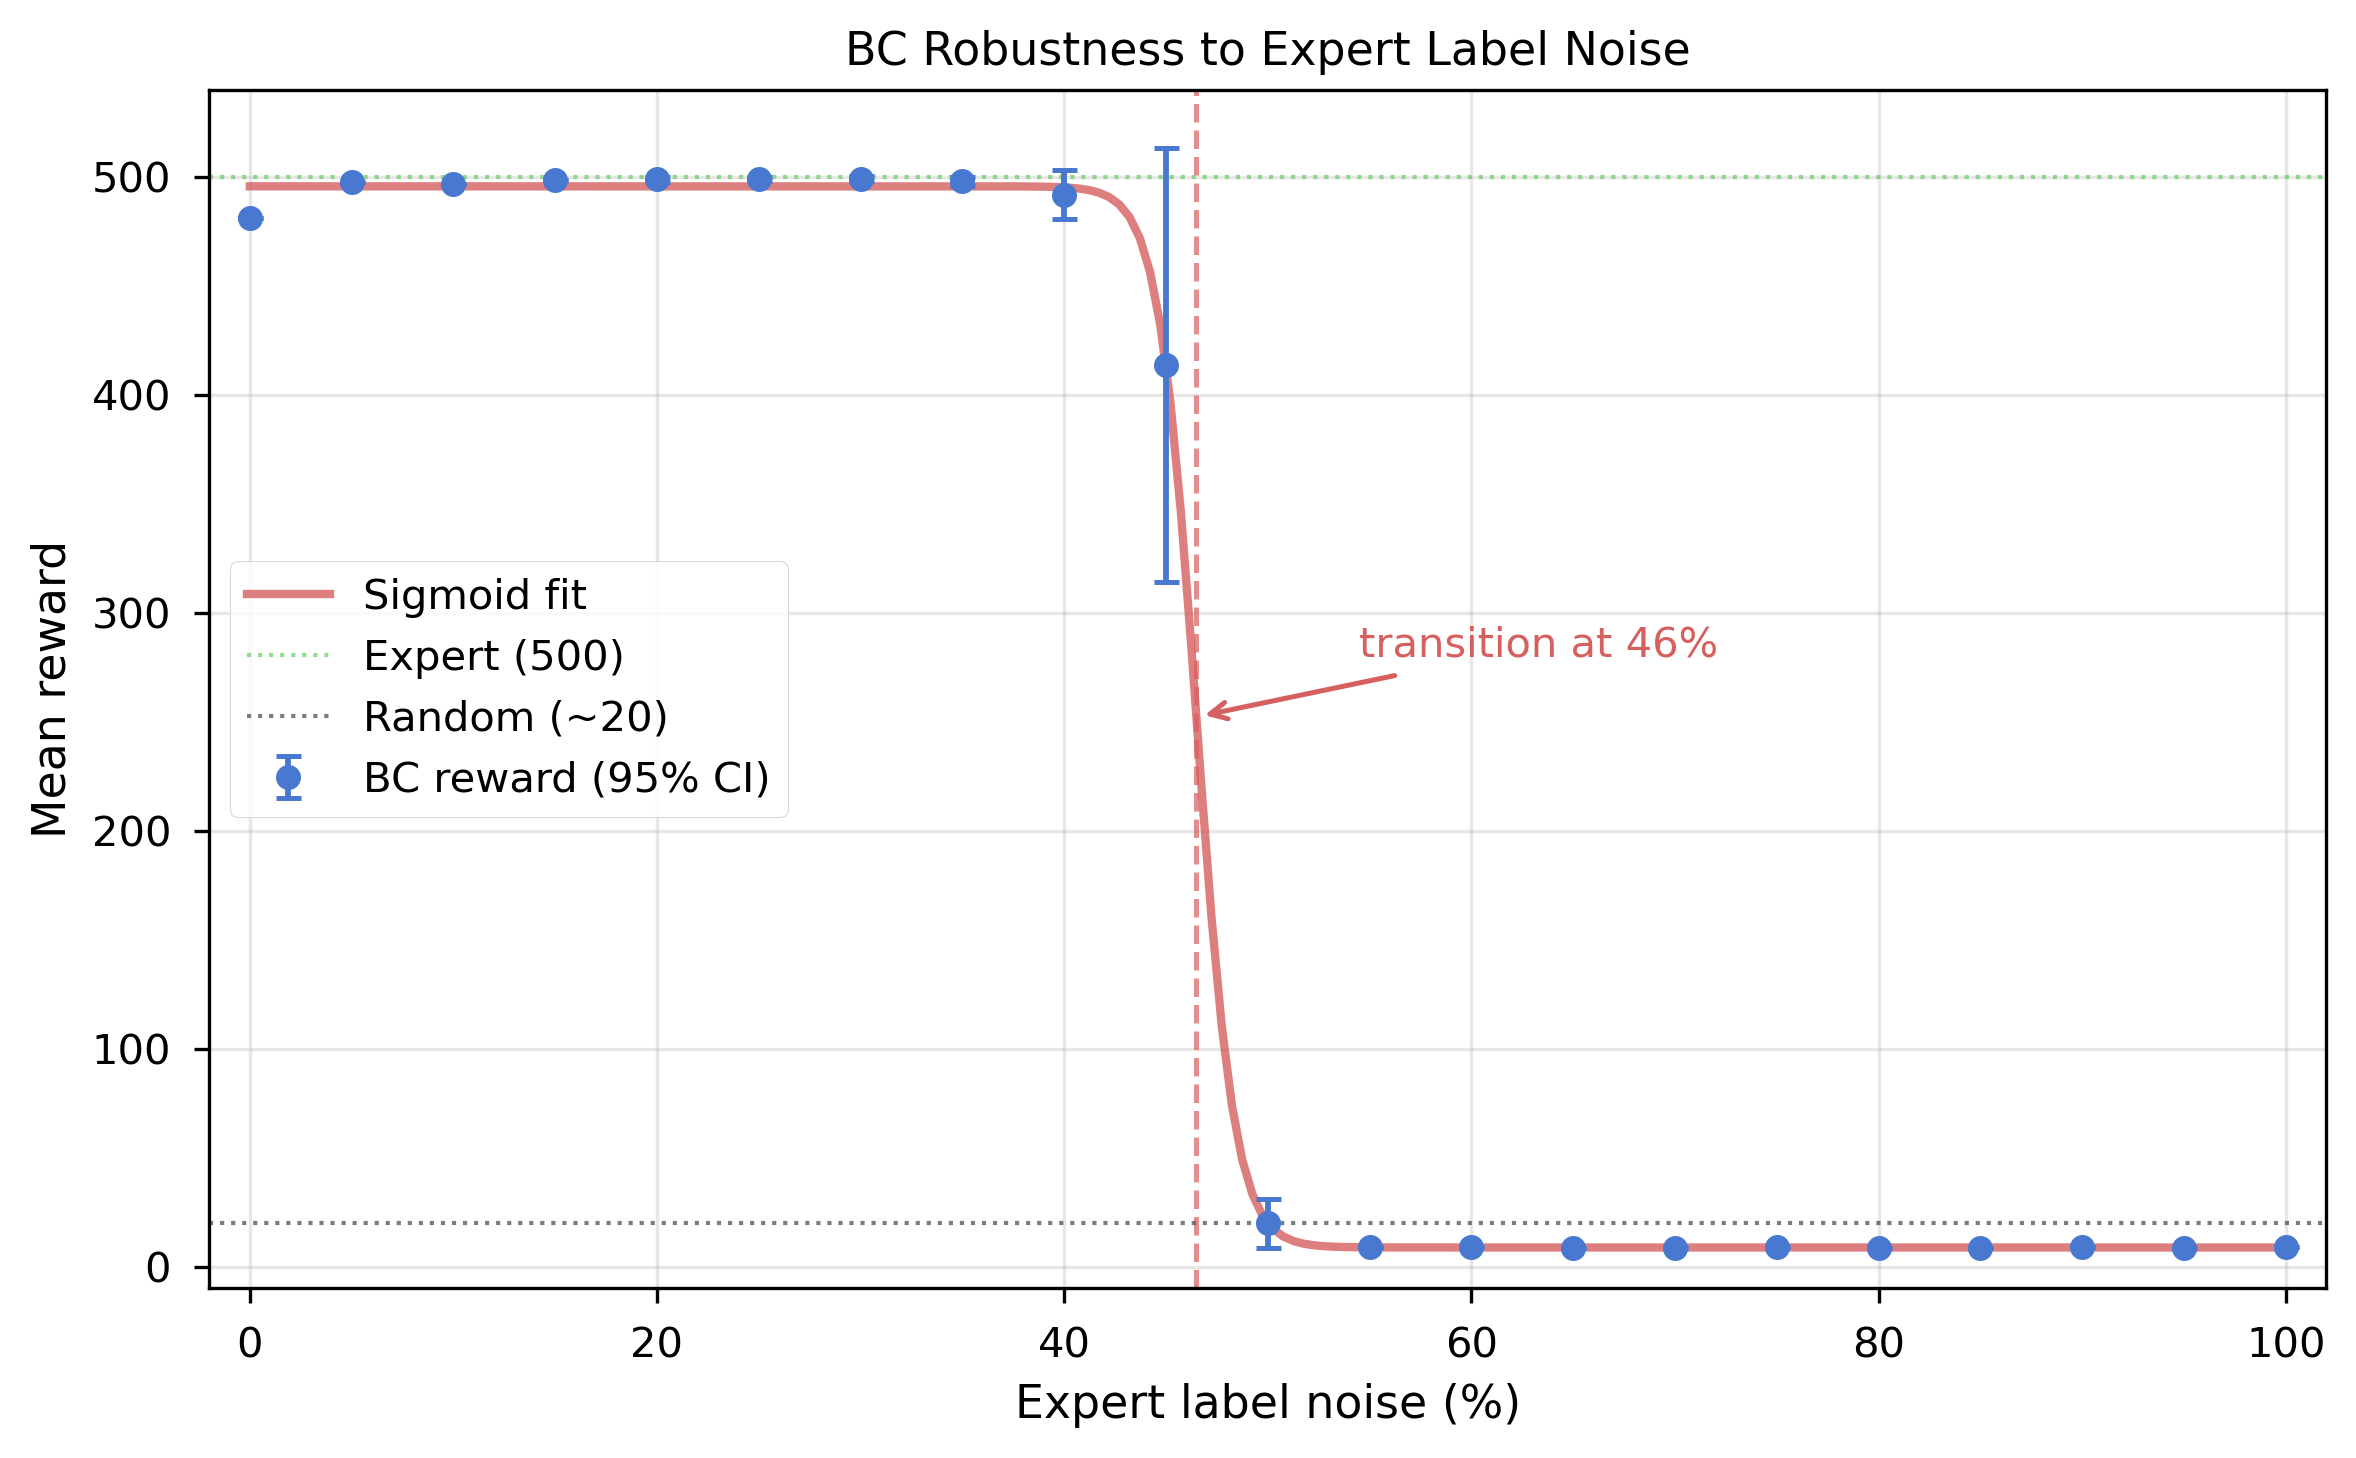
\includegraphics[width=\columnwidth]{figures/fig10_bc_noise_curve.png}
\caption{BC reward vs expert label noise (21 points). Sigmoid fit places the inflection at 46.5\%.
Transition zone (20--50\%) shown with 95\% CIs from 5 seeds.}
\label{fig:bc_noise}
\end{figure}

Three regimes emerge.

\paragraph{Robust regime (0--40\%).}
BC maintains near-perfect performance (reward 481--499) despite up to 40\% of expert actions being flipped.
With binary actions and a clear decision boundary, the majority-vote signal overwhelms noise.

I was surprised to find that 0\% noise (481.1) actually \emph{underperforms} 5\% noise (497.8).
Both are single-seed observations, so I cannot claim significance.
But the direction makes sense as a label-smoothing effect: the expert has systematic preferences in ambiguous states near the decision boundary, and small noise prevents the clone from overfitting to those preferences.

\paragraph{Transition regime (40--50\%).}
Reward collapses from $\sim$492 at 40\% to $\sim$20 at 50\%.
A sigmoid fit gives the inflection at roughly \textbf{46\%} noise (the CI is wide given single seeds outside the transition zone, roughly $[45\%, 48\%]$).
This is slightly below the theoretical 50\% boundary for binary symmetric noise, which makes sense: the MLP needs some margin of signal over noise to learn the boundary.

\paragraph{Anti-correlated regime (50--100\%).}
Above 50\%, reward stabilizes at $\sim$9, consistently below the random-policy baseline of $\sim$20.
The majority of labels are now wrong, so the MLP learns a policy that is systematically anti-correlated with the correct one.
At exactly 50\%, reward $\approx$ 20 (random), confirming the theoretical boundary.

% ===================================================================
\section{Discussion}
\label{sec:discussion}

CartPole turned out to be too simple for most of the techniques I tested.
Baselines don't help, entropy doesn't improve reliability, and gradient variance is the same across methods.
The only intervention that clearly works is RLOO with small $K$, and that is entirely explained by update frequency.

The BC noise experiment was the most interesting part to me: the sigmoid is clean, the transition is sharp, and the hint of a regularization effect from small noise connects to ideas I've seen in ASR label smoothing.

The biggest methodological lesson: I ran 5 seeds, made claims, then ran 15 seeds and had to retract three of them.
I should have started with more seeds.
For binary outcomes like solve/no-solve, 5 runs is just not enough.

% ===================================================================

\end{document}